\chapter{Initializing Vulkan}

\section{Create Vulkan Instance}

To access any of the functionalities offered by Vulkan we first have to create a Vulkan
instance.
To do this we call vkCreateInstance.

\begin{minipage}{\linewidth}{\noindent}
    \lstinputlisting[
        language=C++,
        caption={Create Vulkan instance},
        label={lst::CreateInstance}
        ]{src/ChInitializingVulkan/CreateInstance.cpp}
\end{minipage}

\subsection{VkInstanceCreateInfo}

To call vkCreateInstance we need to pass a pointer to a VkInstanceCreateInfo struct.
This struct collects all the information needed to configure our Vulkan instance.

\begin{minipage}{\linewidth}{\noindent}
\lstinputlisting[
    language=C++,
    caption={VkInstanceCreateInfo initialization},
    label={lst::VkInstanceCreateInfo}
    ]{src/ChInitializingVulkan/VkInstanceCreateInfo.cpp}
\end{minipage}

\subsection{VkApplicationInfo}

We can see that the VkInstanceCreateInfo struct is not the only thing we need.
We have to specify a pointer to a VkApplicationInfo struct. Such struct describes
our Vulkan application.

\begin{minipage}{\linewidth}{\noindent}
    \lstinputlisting[
        language=C++,
        caption={VkApplicationInfo initialization},
        label={lst::VkApplicationInfo}
        ]{src/ChInitializingVulkan/VkApplicationInfo.cpp}
\end{minipage}

\subsection{Layers}

While we initialize our VkInstanceCreateInfo struct, we can specify the layers
that we want to enable.
The specified layers will be loaded after the Vulkan instance creation.

Layers are optional components that hook into Vulkan.
Layers can intercept, evaluate and modify existing Vulkan functions.
Layers are implemented as libraries and are loaded during instance creation.

If we want to enable error checking, we need to load a layer that
provides such functionality.
This kind of layer is know as validation layer.
There are different validation layers.
Here follows an example. Since validation layers cause overhead, we can
disable them when we build the application in release mode.

\begin{minipage}{\linewidth}{\noindent}
    \lstinputlisting[
        language=C++,
        caption={Enabling the Khronos validation layer},
        label={lst::ValidationLayer}
        ]{src/ChInitializingVulkan/ValidationLayer.cpp}
\end{minipage}

\subsubsection{Checking whether our layers are supported}

Before creating our Vulkan instance, we should check if the layers we require are
actually supported.
To do this we use vkEnumerateInstanceLayerProperties.
This function returns all the layers supported by our Vulkan installation.
If all the layers we require are present, then we can proceed to create our
Vulkan instance.

\subsection{Extensions}

While we initialize our VkInstanceCreateInfo struct, we can specify the instance
extensions that we want to enable.
The specified instance extensions will be loaded after the Vulkan instance creation.

Extensions are  additional features that Vulkan implementations may provide.
Extensions add new functions and structs to the API.
Extensions may also change some of the behavior of existing functions.
We can either enable extensions at an instance level or at a device level.

We can use an extension to provide a callback to handle the debug messages
generated by the validation layers.

\begin{minipage}{\linewidth}{\noindent}
    \lstinputlisting[
        language=C++,
        caption={Enabling an extention to handle validation layer debug messages},
        label={lst::DebugExtension}
        ]{src/ChInitializingVulkan/DebugExtension.cpp}
\end{minipage}

We specify one callback that handles messages generated by
instance creation and destruction.
We also specify another callback that handles all other API debug messages.

\begin{minipage}{\linewidth}{\noindent}
    \lstinputlisting[
        language=C++,
        caption={Setting up debug extension callbacks},
        label={lst::DebugExtensionCallbacks}
        ]{src/ChInitializingVulkan/DebugExtensionCallbacks.cpp}
\end{minipage}

The function that creates the VkDebugUtilsMessengerEXT object comes from the
extension we have enabled.
Because of this, we have to load it manually into our address space using
vkGetInstanceProcAddr.
An elegant way to solve this issue us to create a proxy function that handles
this matter for us.

\begin{minipage}{\linewidth}{\noindent}
    \lstinputlisting[
        language=C++,
        caption={Extension function proxy},
        label={lst::ExtensionFunctionProxy}
        ]{src/ChInitializingVulkan/ExtensionFunctionProxy.cpp}
\end{minipage}

\subsubsection{Checking whether our extensions are supported}

Before creating our Vulkan instance, we should check if the instance extensions
we require are actually supported.
To do this we use vkEnumerateInstanceExtensionProperties.
This function returns all the instance extensions that are supported by our
Vulkan installation.
If all the instance extensions we require are present, then we can proceed to
create our Vulkan instance.

\subsection{Vulkan Instance Cleanup}

When our application is shutting down, we need to destroy the debug messenger
and destroy our vulkan instance. DestroyDebugUtilsMessengerEXT is an extension
function proxy.

\begin{minipage}{\linewidth}{\noindent}
    \lstinputlisting[
        language=C++,
        caption={Vulkan Instance Cleanup},
        label={lst::InstanceCleanup}
        ]{src/ChInitializingVulkan/InstanceCleanup.cpp}
\end{minipage}

\section{Open A Window}

After creating our Vulkan instance we need to open a window.
To do this we have two options.
We can use a cross platform library that will do all the heavy lifting
for us, so that we don't have to worry about directly interacting with the OS,
freeing us from the burden of knowing how its windowing API works.
We can also decide to not use a library and opening the window ourselves.
We will do the latter, since it's interesting to know how things work under the surface.

Since I'm on Windows, I'll be dealing with the Win32 API.
We won't go in depth about the specifics of this API since it's beyond our scope.

\subsection{Create Window Handle}

To create a handle to a window we use CreateWindowEx.
We use windowStyle and windowExtendedStyle variables to configure how we want our window.

\begin{minipage}{\linewidth}{\noindent}
    \lstinputlisting[
        language=C++,
        caption={Creating a window handle using Win32 API},
        label={lst::CreateWindowEx}
        ]{src/ChInitializingVulkan/CreateWindowEx.cpp}
\end{minipage}

\subsection{Computing Window Dimensions}

Before creating our window, we need to compute its width and height.
This is due to the fact that a window comprises of a client area and a non client area.
We usually want our client area to be of a certain size, but CreateWindowEx takes
the whole window width and the whole window height as arguments.

\begin{figure}[ht]
    \centering
    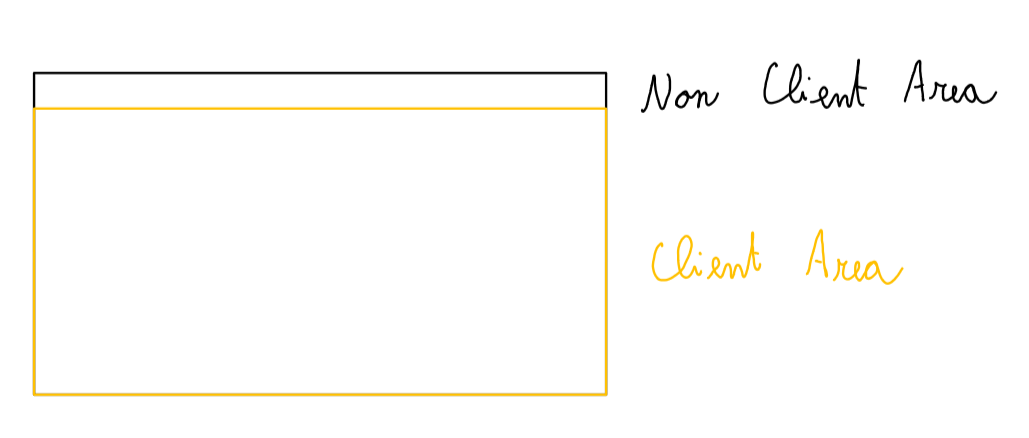
\includegraphics[scale=0.30]{images/ChInitializingVulkan/Win32Window.png}
    \caption{Anatomy of a Win32 Window}
    \label{fig::Win32Window}
\end{figure}

\begin{minipage}{\linewidth}{\noindent}
    \lstinputlisting[
        language=C++,
        caption={Compute window width and height},
        label={lst::AdjustWindowRectEx}
        ]{src/ChInitializingVulkan/AdjustWindowRectEx.cpp}
\end{minipage}

\subsection{Register Window Class}

Before creating our window, we need to register its window class.
To do this we use RegisterClassEx.
This function takes a pointer to a WNDCLASSEX struct.
This struct is used to configure our window class;

\begin{minipage}{\linewidth}{\noindent}
    \lstinputlisting[
        language=C++,
        caption={Register Window Class},
        label={lst::RegisterClassEx}
        ]{src/ChInitializingVulkan/RegisterClassEx.cpp}
\end{minipage}

\subsection{Window Procedure}

While filling in our WNDCLASSEX struct, we also passed a WindowProcedure.
This is a callback function that we have to define.
We use this function to handle the events that our window will receive during
the lifespan of our application.

The Win32 API also provides a default window procedure.
Our custom window procedure will call this default procedure when we don't want
to handle particular events ourselves.

\begin{minipage}{\linewidth}{\noindent}
    \lstinputlisting[
        language=C++,
        caption={Window Procedure},
        label={lst::WindowProcedure}
        ]{src/ChInitializingVulkan/WindowProcedure.cpp}
\end{minipage}

\subsection{Window Cleanup}

When our application is shutting down, we need to destroy our window and unregister
its class.

\begin{minipage}{\linewidth}{\noindent}
    \lstinputlisting[
        language=C++,
        caption={Window Cleanup},
        label={lst::WindowCleanup}
        ]{src/ChInitializingVulkan/WindowCleanup.cpp}
\end{minipage}

\section{Create A Presentation Surface}

We need to link our newly created window to our Vulkan instance.
To do this we need to create a presentation (or window) surface.
This operation is platform specific.
Since we are using Windows, to create our presentation surface we need
to use vkCreateWin32SurfaceKHR.

\begin{minipage}{\linewidth}{\noindent}
    \lstinputlisting[
        language=C++,
        caption={Create Presentation Surface},
        label={lst::CreatePresentationSurface}
        ]{src/ChInitializingVulkan/CreatePresentationSurface.cpp}
\end{minipage}

\subsection{VkWin32SurfaceCreateInfoKHR}

When we call vkCreateWin32SurfaceKHR, we need to pass a pointer to a
VkWin32SurfaceCreateInfoKHR struct.
Such struct lets us configure our presentation surface creation.

\begin{minipage}{\linewidth}{\noindent}
    \lstinputlisting[
        language=C++,
        caption={Filling in a VkWin32SurfaceCreateInfoKHR struct},
        label={lst::VkWin32SurfaceCreateInfoKHR}
        ]{src/ChInitializingVulkan/VkWin32SurfaceCreateInfoKHR.cpp}
\end{minipage}

\subsection{Required Instance Extensions}

Vulkan, being cross platform, cannot interact directly with the OS windowing system.
To do this we need to use extensions.

The first extension that we need to enable is the instance level KHR surface extension.
This extension exposes a VkSurfaceKHR object that represents a surface to present
rendered images to.
This surface will be backed by the window we have created.

The second extension we need to enable is platform specific and is needed
to create our VkSurfaceKHR object.
In our case, since we are using Windows, we need to enable the instance level KHR win32
surface extension.

\begin{minipage}{\linewidth}{\noindent}
    \lstinputlisting[
        language=C++,
        caption={Presentation Surface Extensions},
        label={lst::PresentationSurfaceExtensions}
        ]{src/ChInitializingVulkan/PresentationSurfaceExtensions.cpp}
\end{minipage}

Notice the define preprocessor directive right before including our Vulkan header.
We need to do this to access our native platform functions.

\subsection{Presentation Surface Cleanup}

When our application is shutting down, we need to destroy our presentation surface.

\begin{minipage}{\linewidth}{\noindent}
    \lstinputlisting[
        language=C++,
        caption={Presentation Surface Cleanup},
        label={lst::PresentationSurfaceCleanup}
        ]{src/ChInitializingVulkan/PresentationSurfaceCleanup.cpp}
\end{minipage}

\section{Pick A Physical Device}

\section{Create A Logical Device}

\section{Create A Swapchain}
